\documentclass[letterpaper,twocolumn,10pt]{article}
\usepackage{usenix2019_v3}

% to be able to draw some self-contained figs
\usepackage{tikz}
\usepackage{pgfplots}
\usepackage{amsmath}


%-------------------------------------------------------------------------------
\begin{document}
%-------------------------------------------------------------------------------

%don't want date printed
\date{}

% make title bold and 14 pt font (Latex default is non-bold, 16 pt)
\title{\Large \bf Software Security Analysis of Ethereum Smart Contracts}

\author{
{\rm Nicolas Schapeler}\\
TUM Chair of IT Security
} % end author

\maketitle

%-------------------------------------------------------------------------------
\begin{abstract}
The Ethereum blockchain allows for the decentralized execution of code using so-called smart contracts, which are already being leveraged for a variety of applications. However, this new technology also comes with new security vulnerabilities, which have already been exploited in the past and caused millions of USD in financial damage.
To avoid such attacks in the future to the best of our abilities, we present Ethereum-specific software security analysis methodologies and tools. We begin by introducing static analysis approaches such as Symbolic Analysis, then continue by presenting dynamic detection tools employing local simulations of the blockchain. We finalize our systemization of knowledge by comparing a set of the tools presented in regards to their performance in order to determine the fastest currently available implementation.


\end{abstract}


%-------------------------------------------------------------------------------
\section{Motivation}
%-------------------------------------------------------------------------------
In recent years blockchain technology has seen more and more widespread adoption, ranging far from its initial use case of a decentralized means to exchange electronic cash, as introduced by Bitcoin \cite{nakamoto}.

A key innovation in this space has been the introduction of so-called smart contracts, which were first implemented by the Ethereum protocol based on the ideas of Nick Szabo \cite{szabo_1996}. These are programs that execute automatically on the Ethereum network if certain conditions are met or if they are invoked by a blockchain participant. Through these, one can create more complex applications while still retaining the built-in trustlessness and security for which blockchain technology was initially designed. Today, smart contracts are used to automate various processes, ranging from supply chain management \cite{bhandari_2018} over energy distribution in smart grids \cite{giannakaris_trakadas_zahariadis_gkonis_papadopoulos_2019} to health care \cite{griggs_ossipova_kohlios_baccarini_howson_hayajneh_2018}.

The use case that provides the main motivation for this paper, however, is Finance. Here smart contracts are used to automate and enforce financial agreements between different parties, such as loan provisions, asset exchanges, and asset management amongst others. At the time of this writing, four of the top smart contracts on the Ethereum network manage around 60 Billion USD \cite{nr1} \cite{nr2} \cite{nr1T} \cite{nr2T}, with hundreds of other contracts overseeing multiple millions in value. Considering this in addition to the relative novelty of the field to both developers and law enforcement along with the built-in anonymity of blockchain technology applications, one can deduce why this field presents such an attractive target to malicious actors. At its current stage, performing an attack on a smart contract application often yields extremely high rewards in comparison to the risk of facing consequences.

For these reasons, smart contracts have been the target of multiple high-profile attacks in the past years. The first large-scale attack was the DAO-Attack in 2016, where 3.6 Million Ether, worth around 50 Million USD at the time or 10 Billion USD today,  was stolen and lead to the developers of Ethereum taking the controversial action of manually reverting the attacker's exploit transactions \cite{atzei_bartoletti_cimoli_2017}. Other prominent attacks include the King of the Ether Throne attack in 2016 and the Parity Multisig Wallet Attack in 2017 \cite{atzei_bartoletti_cimoli_2017} (more details regarding the exact exploits used in these attacks are given in the Background). The reason we mention these specific attacks is that all of them exploited vulnerabilities that in hindsight appear relatively simple. The key significance, however, is that the vulnerabilities utilized are all smart contract-specific, and may therefore not be intuitively detected by a developer with lesser experience developing such applications. As previously mentioned, due to the relative novelty of smart contracts, few developers are highly experienced and are therefore prone to fall victim to already-known vulnerabilities. For this reason, we believe the software security analysis methodologies and tools disclosed in this paper are of key importance in a space where each security flaw can lead to significant financial loss: They allow for the detection of vulnerabilities the developer may not be aware of or may have overlooked.

This Systemization of Knowledge begins by giving a brief overview of the background concepts regarding software security analysis and Ethereum smart contracts, followed by a systemization of different approaches to security fault detections, where we present and experimentally test the performance of various existing tools.


%-------------------------------------------------------------------------------
\section{Background}
%-------------------------------------------------------------------------------
In this section, we provide the theoretical background information related to software security analysis and Ethereum necessary for understanding the rest of this paper.

\subsection{Ethereum}
Ethereum is an open software protocol that allows for the decentralized execution of smart contracts and the exchange of value in its native cryptocurrency, Ether \footnote{Technically the unit smart contracts and accounts exchange value in is Wei, however we use Ether in the context of this paper as this makes the numbers far more manageable ( 1 Ether = $10^{18}$ Wei). }.  These smart contracts run on the Ethereum Virtual Machine (EVM). The specification of the Ethereum protocol and the EVM is precisely explained in Wood's Ethereum yellowpaper \cite{wood_2021}. We provide a shortened overview based on his work below:

\subsubsection{EVM}

The Ethereum Virtual Machine is a distributed state machine with its own set of instructions and own state at any given time. This state records all relevant information related to the Ethereum network. As one might expect, the EVM's role is to define a state transition function using its instruction set which clearly defines which next state is reached given an input state and a certain instruction to be executed.

\subsubsection{Accounts and Smart Contracts}


In this context, a significant data structure for the Ethereum protocol is the account. This data structure has the ability to send and receive transactions, hold a balance of Ether, and interact with other smart contracts. We differentiate between two types of accounts, externally-owned accounts and smart contracts. Externally-owned accounts are generated using a public-private key-pair and can interact with the rest of the Ethereum Network using the private key's signature as proof that an instruction stems from a specific account. These signed EVM instructions that accounts use to interact with one another are called transactions.  Smart Contracts, on the other hand, are deployed as pieces of software and do not come with a private-public key pair. They define a set of callable functions that other network participants can invoke. As such, a key difference between smart contracts and externally-owned accounts is that smart contracts can only perform transactions if they were first invoked by a different account. As smart contracts can be called by any account (both externally owned and other smart contracts) on the Ethereum network, it is crucial that all network participants agree what a smart contract can and cannot do. To enforce this, the code of smart contracts is strictly immutable \footnote{To be clear, only the code of smart contracts is immutable. Smart Contracts can still contain various data structures such as variables, mappings, arrays etc. which are mutable.}.

\subsubsection{Gas Fees}
\label{subsection:gas}

As previously mentioned, the physical hardware the EVM runs on and transactions are executed on is provided by a subset of all network participants, called nodes. Since these do not want to give storage and computing power away for free, Ethereum implements a gas system, whereby each operation offered by the EVM is assigned a certain gas cost \footnote{It should be noted that taking up memory also has a certain gas cost which scales with the amount of memory taken up. This has the consequence that smart contracts are often tried to be written as concisely as possible as to avoid any unnecessary memory takeup when deploying its code onto the network and therefore spending.}. This gas is just a fee in Ether paid for the computing effort and/or storage provided by the nodes. It is important to note that the maximum an account is willing to pay for these gas fees is set by the transaction initiator, not the processing nodes. The nodes, however, have the choice of processing transactions in whatever order they please and will usually choose transactions with the highest fees and lowest effort to themselves. This means a transaction can take a significant amount of time to be processed or be rejected by the nodes altogether if the nodes believe the fees are not high enough for their expended effort. It is also to be noted, that blocks in the Ethereum Network have an upper gas limit, a limit on how much computation can be done and how much gas can be spent in one block, which can also lead to a transaction being reverted if the work performed in it costs more gas than the upper gas limit.

\subsection{Solidity}
\label{subsection:sol}
Although the smart contract representation one finds on the physical blockchain is in EVM bytecode, very few smart contracts are manually written in this form and instead employ higher-level languages. There are multiple programming languages specifically adapted for developing smart contracts, however, in the context of this paper, we set our focus on Solidity. The reason we choose this language is not only for it being the most popular \cite{gebele_2020} but also due to it having received criticism for being designed in a way that facilitates errors that lead to security flaws in smart contract development\footnote{This can partially be seen by the long list of pitfalls provided by the official documentation\cite{ethereumrevision0bbfe453}.}. We introduce some of these patterns here in addition to other Ethereum-specific security vulnerabilities in order to better help the reader's understanding of the types of issues the software security analysis tools detect in the Contribution section of this paper.

\begin{itemize}
  \item \textbf{Inconsistent Exception handling}

	Exceptions can be caused by various factors, such as a transaction going over its allocated gas fee limit, the EVM call stack overflowing, or the \verb|throw| command being called. However, when an exception is raised, Solidity is not consistent in how it handles these and may therefore facilitate creating vulnerabilities caused by incorrectly handling exceptions. For example, if one wants to transfer Ether from an account to another, this can be done in 3 ways:
	\begin{enumerate}
	\item \verb|<receivingAddress>.transfer(amount)|
	\item \verb|<receivingAddress>.send(amount)|
	\item \verb|<receivingAddress>.call().gas().value(amount)|
	\end{enumerate}

	These have some key differences: The \verb|transfer| method throws an exception if the transfer fails for any reason and reverts the entire transaction it was a part of. The other two, however, simply return \verb|False| on failure and do not revert the transaction. Additionally, \verb|transfer| and \verb|send| have a fixed gas fee when used, while \verb|call| can have its gas fee set by the invoker \footnote{Though we use $call$ and $send$ in this context to transfer funds, the main use of these commands is to invoke a function in a smart contract.}.
  \item \textbf{Fallback function}

  Smart contracts have the option of defining a so-called fallback function which is executed when receiving Ether without the sender specifying a function call \footnote{If a contract does not define such a function, it cannot receive Ether.}. Aside from being executed as a side effect to receiving Ether, this function is also executed in other situations that may seem unexpected. Given a contract $C$ with a function with the signature \verb|function f(uint) returns (byte)|, if one were to call the function \verb|function f(int) returns (byte)| (notice the incorrect signature) on $C$, the result would not be a revoked transaction, exception, or a returned \verb|False| boolean, but rather an execution of the fallback function of $C$. The same is true if one mistypes the address of $C$ and attempts to invoke the nonexistent function \verb|f| on a contract $C'$, the result is an execution of the fallback function of $C'$.

  This behavior worked in conjunction with the exception handling inconsistencies to cause the King of the Ether Throne attack mentioned in the introduction \cite{atzei_bartoletti_cimoli_2017}. There, the essence of the attack was invoked through the usage of the previously introduced \verb|send| function in the vulnerable contract. The intention of \verb|send| in the victim contract was to simply send an amount of Ether to an address, however the programmer had forgotten about the side-effect of the invoked fallback function if the recipient is a contract. Next, the \verb|send| function's fixed gas fee was not enough to pay for the attacker's contract's fallback function fee and an exception was produced, which \verb|send| returns through the use of a boolean. The victim contract, however, had no boolean check for \verb|send|, which resulted in the victim contract finding itself in a deadlocked state.

    \item \textbf{Reentrancy}


    This vulnerability is not as much an influence of Solidity's design like the previous two examples, however we view it as one of the key attack vectors in smart contract development and therefore provide a short explanation. Assume we have two Smart Contracts:

  \begin{verbatim}
contract Bank{
  mapping (address => uint) balances;

  function withdraw(uint _val) public {
    // msg.sender is the account that
    // made the function call
    address a = msg.sender;
    // Check sufficient balance
    if(balances[a] >= _val) {
      // Send the money
      // and check the send succeeded
      require(a.call.value(_val).gas());
      // Remove sent money from balance
      balances[msg.sender] -= _val;
      }
   }
}

contract Attacker{
  // Fallback function,
  // executed when receiving money
  function() payable {
    // Call Bank.withdraw again
  }
}
  \end{verbatim}

As one can deduce from the provided code, the vulnerability here is that the bank first sends money to the withdrawing account before removing the sent money from the account's balance. Additionally, the bank uses the \verb|call| function to send money and does not specify a maximum gas fee. An attacker can therefore implement a more complex fallback function without the risk of their money transfer failing due to the gas fee of their fallback function being too high. The attacker leverages this by calling the withdraw function again, thereby being able to withdraw as much money as he wants from the bank contract until the bank is out of money. This sort of vulnerability is what was leveraged in the DAO Attack mentioned in the introduction \cite{atzei_bartoletti_cimoli_2017}.

    \item \textbf{Transaction Order Dependence}

    As explained in Section~\ref{subsection:gas}, one cannot predict the order in which transactions arrive with 100\% accuracy, as it is the processing nodes that determine which transactions they choose to handle first. This situation is comparable to race conditions in other types of programming. If a contract is dependent on the order in which transactions arrive in spite of this and does not implement a way to handle this indeterminism, one can easily construct examples where this could lead to unexpected behavior, especially if one considers every transaction can be read by the processing nodes prior to their execution. For example, consider a contract that sells an asset, where Alice is the owner of said asset and Bob is the buyer. Bob sends a transaction to buy the asset at the time where it costs 1 Ether. Alice sees this transaction prior to being processed and quickly sends off a transaction setting her assets price to 100 Ether. With a high enough gas price or large enough control over the processing nodes, Alice can ensure her transaction arrives prior to Bob's, draining Bob of 99 more Ether than he had planned to pay originally.




	\item \textbf{Denial of Service (DoS) using Gas Limit}

	The final attack vector we seek to present is a DoS attack, based on Atzei et al.'s 2017 SoK of Ethereum Attacks \cite{atzei_bartoletti_cimoli_2017}. Assume we have given the following contract:

\begin{verbatim}
contract DoS{
  address[] ads;

  function addAdr(address toAdd) {
    ads.push(toAdd);
  }

  function f(){
    for(uint i = 0; i < ads.length; i++) {
        // Some operation on each address
    }
  }
}
\end{verbatim}

An attacker can provoke a DoS by adding suficiently large number of addresses to the \verb|ads| array of the contract. Then, if another account seeks to execute \verb|f|, the gas cost will be so high that it surpasses the block gas limit and the execution will fail.

  \end{itemize}

\subsection{General Security Analysis Methodologies}

Finally, we introduce some general security analysis methodologies which adaptions to Ethereum will be presented in Section 3 of this paper.

\subsubsection{Symbolic Execution}

Symbolic Execution takes a program's source code as an input and assigns symbolic values to unknown inputs. It then executes the given program using said symbolic values and is thereby able to compute expressions for the unknown inputs along with fitting constraints belonging to each possible execution path of a program. These constraints can then be solved to determine a concrete input that leads to the execution of a given path. This is usually done with the help of an SMT (Satisfiability modulo theories) solver which can  determine if a given first-order logical expression is satisfiable. An example of such a solver is the Z3 Solver developed by Moura and Bjorner \cite{moura_bjorner_2008}. A key limitations of Symbolic Execution is path explosion, where the number of possible paths to symbolically execute becomes very big very quickly for large programs, especially if these contain loops that cannot be trivially rolled out. Additionally, operating system models such as file systems can also prove to be difficult to simulate.

\subsubsection{Symbolic Model Checking}
The general idea of Model Checking is to generate the set of states a program can reach and to verify wether a set of given properties hold true in each of these states \cite{osterland_rose_2020}. If a state is found that violates a property, an example to reach this state is usually provided for debugging. Like Symbolic Execution, a key weakness of this approach is state space explosion; the number of reachable states grows very fast when the size of the code to be analyzed becomes larger. Symbolic Model Checking is a method to somehwat mitigate this issue, as it represents each state not as explicit values but rather as logical formulas  or similar data structures representing a set of equivalent inputs.

\subsubsection{Taint Analysis}
Taint Analysis focuses on tracking data inputted by users and verifying if it is properly sanitized as to prevent harm to the system accepting it.

\subsubsection{Mutation Testing}
\label{subsection:mut}
The goal of Mutation Testing is to assess the efficiency of the test suite belonging to a certain piece of software. It works by generating so-called "mutants" of the provided source code, which are clones of the original code with slight alterations (for example, a change from a $>$ to a $\geq$). Then, the given test suite is ran on these generated mutants and the amount of mutants that pass the tests is measured. Generally, a low amount of mutants passing all tests is viewed as evidence of the test suite's high quality.

\subsubsection{Fuzzing}
Fuzzing is a process whereby random and/or purposefully invalid data is input into a program one seeks to test and the program is monitored for unexpected behavior, such as crashes or exceptions.

%-------------------------------------------------------------------------------
\section{Security Analysis Methodologies}
%-------------------------------------------------------------------------------
In this section we present current methodologies for detecting security analysis of smart contracts, where we split the approaches into two camps; static and dynamic methodologies.


\subsection{Static Analysis Methods}
We define static analysis as analysis performed on smart contract code or bytecode in a non-runtime environment without direct execution of the given smart contract.


Due to the general difficulty of realizing a realistic simulation of the runtime environment of smart contracts, there is a wide array of static analysis methods. One of the reasons for this difficulty is that some Ethereum-specific security flaws stem from the outcome of operations which are dependent on arrival times of transactions on the blockchain. As established earlier, the order of these is determined by the nodes on the network and is therefore non-deterministic. Additionally, many smart contracts interact with other smart contracts and writing stubs for all of these can prove to be very time-consuming and in some cases, unfeasible. Note that each of the headings from here on refer to the usage of a specific technique in the context of Ethereum as opposed to its usage in general, as was the case in the previous section.


\subsubsection{Symbolic Execution}
A technique commonly found in various automated software security analysis engines is Symbolic Execution. Symbolic Execution provides the advantage of analyzing contract code based on available paths rather than available inputs. The amount of possible paths are often easier to generate than inputs that, depending on order, lead to differing outcomes.

Furthermore, smart contracts generally mitigate some of the weaknesses of Symbolic Execution mentioned earlier: First, they are generally kept rather short, as each additional unit of memory comes with a certain gas cost when deploying onto the Ethereum network. Next, smart contracts often avoid unbounded/unconstrained loops, as these can also pose a security risk and lead to potential DoS attacks, as explained in Section ~\ref{subsection:sol}. Additionally, compared to a regular computer, the EVM is comparatively simple to simulate, as it does not have many operating system-like features.


One of the first tools to utilize this was OYENTE which was introduced by Luu et al. \cite{luu_chu_olickel_saxena_hobor_2016}. OYENTE can detect 4 types of security weaknesses: Transaction Ordering Dependences (TOD), Timestamp Dependences \footnote{This vulnerability simply refers to a contract that executes based on the block timestamp. The reason this is insecure is because the node that processes the block can vary the timestamp by up to 900 seconds from the real system time and could thereby influence the contract execution in their favor.}, Exception Mishandling, and Re-entrancy vulnerabilities. OYENTE takes two inputs, namely the EVM bytecode of the contract to be analyzed and the current global state of the Ethereum Network. Here, the latter input is used to initialize certain contract variables from the bytecode in order to ensure a more accurate base state to perform Symbolic Execution from. The tool thereby leverages the availability and accessibility of both these inputs, as both are stored on the Ethereum blockchain and can be obtained using most Ethereum block explorers for any given smart contract.

\begin{figure}
\begin{center}
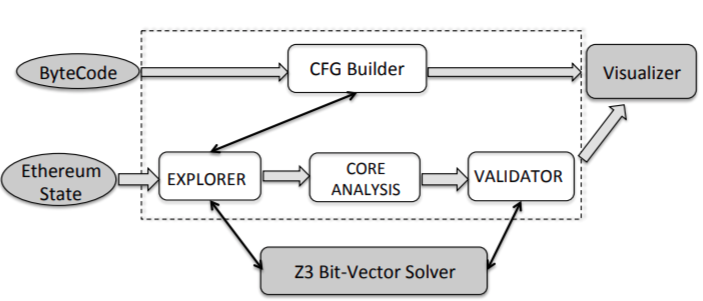
\includegraphics[scale=0.35]{oyente}
\end{center}
\caption{\label{fig:oyente} The OYENTE Tool's Structure \cite{luu_chu_olickel_saxena_hobor_2016}}
\end{figure}


OYENTE works in 4 steps, depicted in Figure~\ref{fig:oyente}: First, it generates a control flow graph (CFG) of the smart contract at hand. Next, the Explorer component iterates over all symbolic states\footnote{Or until a pre-defined execution time limit is reached.}, starting with the entry node of the CFG. In each of these states the Explorer then symbolically executes a single instruction. If such an instruction is a branching conditional, the Explorer queries the Z3 constraint solver \cite{moura_bjorner_2008} to determine if either of the possible paths is provably impossible to reach, in which case that path is ignored. If not, both paths are explored in a depth-first manner. This exploration produces a set of symbolic traces along with fitting path constraints and other data used in later steps. The output of this operation is then scanned for the previously defined security vulnerabilities. This is done by checking for certain patterns in the symbolic trace \footnote{For example, to find if the contract mishandles exceptions, it is verified in the symbolic trace that everytime an exception is thrown and the contract pushes a boolean to the stack, the contract also performs a check for that boolean right after. This sort of detection is the general idea for the other 3 patterns as well, however closer explanation would go outside the scope of this paper.}. In the final analysis step, Validation, the detected vulnerable traces are checked using the Z3 solver to ensure that they are provably reachable, thereby eliminating false positives \footnote{The authors warn, however, that the validator is "far from being complete" \cite{luu_chu_olickel_saxena_hobor_2016}.}. Finally, the result is displayed to the user. OYENTE is specifically highlighted in this paper, as it was one of the first checkers in the space and designed with extendability in mind, serving as the base for multiple others \cite{zhou_hua_pi_sun_nomura_yamashita_kurihara_2018}\cite{albert_gordillo_livshits_rubio_sergey_2018}. A particularly interesting extension of OYENTE is Chen et al.'s GASPER \cite{chen_li_luo_zhang_2017}, which uses OYENTE as a base to detect code that uses an unnecessarily high amount of gas \footnote{Unregulated gas spend can lead to unintended behavior of the smart contract if not handled adequately and can be exploited by a malicious actor to manipulate the smart contract in his favor, for examply by provoking a DoS attack as presented in section \ref{subsection:sol}.} and identifies a set of gas costly patterns defined by the authors.

 A different software security analysis tool that uses Symbolic Execution is Mythril by Mueller et al. \cite{mueller}. The general functionality of Mythril is rather similar to that of OYENTE, however a significant advance Mythril made over OYENTE is in deciding which paths are feasible during its equivalent of OYENTE's Explorer phase\footnote{Another key improvement of Mythril is its ability to detect so-called trace vulnerabilities. This is not further elaborated here in order to avoid redundancy, as this topic is discussed in depth in Section~\ref{subsection:trace}.}. Aside from using the Z3 solver to determine if a path is reachable, Mythril also introduces a variety of other ways to reduce the number of paths explored in an update to the original paper co-authored by Luca \cite{mueller_luca_2019}:

\begin{enumerate}
	\item Pure functions

	If a function has no side effects and is deterministic, we call it a pure function. As the execution of such a function has no effect on the state of the smart contract it is invoked on, Mythril filters these out of their paths when performing Symbolic Execution.

	\item First encounter


	When encountering a new path to execute, Mythril verifies if the path has been executed before and only follows it if that is not the case.

	\item Variable Edited

	Mythril only executes a path if this path reads a variable that was edited elsewhere or if this path writes a variable that is read elsewhere.

	\item Directed Execution

	This method allows an outside party to give the Symbolic Execution tool information about certain variables (e.g. ranges for integers) and to specify parts of the code where Symbolic Execution is not needed.

	\item State merging

	After a Symbolic Execution step takes place, merge states together by concatenating their constraints together using a logical \verb|OR|. This approach is not used by Mythrill, but has been implemented in other tools \cite{mossberg_manzano_hennenfent_groce_grieco_feist_brunson_dinaburg_2019}.


\end{enumerate}

\subsubsection{Generic Property Verifiers}
Symbolic Analysis tools as presented in the previous section have room for extension, as they are  limitated to only detecting the security flaws that are hard-coded into them. However, as time passes and the Ethereum ecosystem grows, new security flaws are discovered which one wants to check for as well. The developers of OYENTE heeded this fact when they originally designed it by allowing for simple extendability. However, this still requires one to manually program an extension for OYENTE if one desires to verify a specific property that is not part of the original implementation of OYENTE. Therefore, property verifiers that take in some form of security policy were developed.


An example of such a generic property checker is ZEUS by Kalra et al. \cite{kalra_goel_dhawan_sharma_2018}, which takes in the Solidity source code of a given smart contract along with a policy specification of properties to test and uses Symbolic Model Checking to verify these. Broadly speaking, ZEUS works by collecting the constraints and their auxiliary information in the XCAML (eXtensible Access Control Markup Language) format. Next, it translates the source code to an abstract contract language introduced in the paper and, using the XCAML representation, inserts the predicates specified by the policy into this code using \verb|assert| statements. This \verb|assert|-enhanced code is then translated to LLVM (Low Level Virtual Machine) \cite{lattner_adve} byte code. Finally, ZEUS uses a symbolic model checker to to verify that each of the conditions specified in the policy and therefore represented by an \verb|assert| statement holds true. The checker used in ZEUS is SeaHorn \cite{gurfinkel_kahsai_komuravelli_navas_2015}, however ZEUS is compatible with any checker that operates on LLVM code. Additionally, the authors claim ZEUS is significantly faster than OYENTE in addition to detecting fewer false positives.


A further contribution in this field was Securify introduced by Tsankov et al. \cite{tsankov_dan_drachsler-cohen_gervais_bünzli_vechev_2018}.  Similar to ZEUS, Securify takes in two inputs, the contract code as EVM bytecode and a list of insecure semantic patterns to scan for. First, it transforms this EVM bytecode into a stackless representation in static single assignment (SSA) \footnote{This is an intermediate form with two properties, each variable is only assigned once and each variable has to be defined before being used.} form. Once this form has been reached, Securify scans it for semantic facts, such as control-flow dependencies between two variables. These semantic facts are saved in stratified Datalog. The advantage of doing this, is that this representation can be compared to the provided security patterns using existing Datalog solvers. A key improvement the authors of Securify sought to make over ZEUS was the introduction of violation patterns, whereas ZEUS only supports compliance patterns. Given a certain security property, a compliance pattern is defined as an implication for this property to be satisfied, whereas a violation pattern implies this property to not be satisfied.


\subsubsection{Formal Verification}
A different approach to static analysis is through means of formal verification and theorem provers.

\begin{figure}
\begin{center}
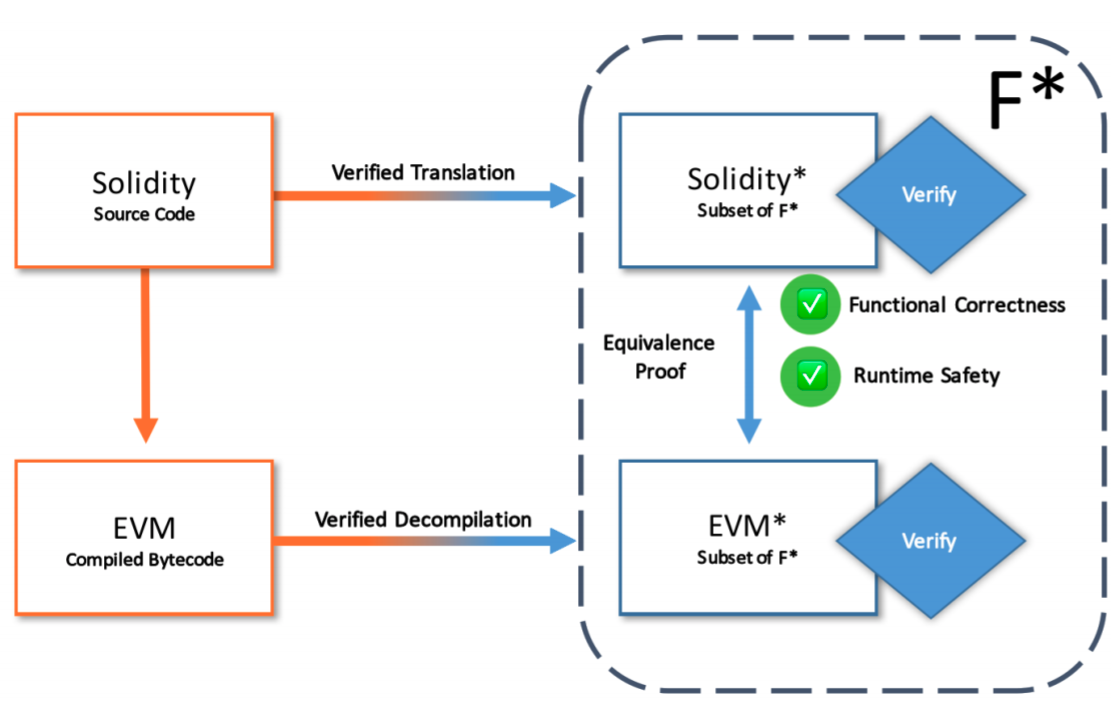
\includegraphics[scale=0.2]{Fstar}
\end{center}
\caption{\label{fig:fstar} The F* Tool's Structure\cite{bhargavan_delignat-lavaud_fournet_gollamudi_gonthier_kobeissi_kulatova_rastogi_sibut-pinote_swamy_etal._2016}}
\end{figure}


One example is the F*-Framework by Bhargavan et al. \cite{bhargavan_delignat-lavaud_fournet_gollamudi_gonthier_kobeissi_kulatova_rastogi_sibut-pinote_swamy_etal._2016}. The authors aim to ensure the functional correctness and runtime safety of a given Solidity smart contract. The paper proposes an architecture of two translators, one taking in Solidity Code, and one taking in EVM Bytecode. This setup is visualized in Figure~\ref{fig:fstar}. Each of these translators translates their input into the functional language F*. Once a representation in F* is obtained, functional correctness checks can be performed on certain properties \footnote{The authors only mention checking for a valid gas limit in their paper.} which are verified by a SMT solver \footnote{The SMT solver can be applied to queries generated from F*'s "rich type system" and "monadic effect", however the authors do not explain how this works in more detail.}. In the rare case (the authors claim this is the case for only 396 out of 112,802 contracts on Etherscan) where both the Solidity Code and EVM Bytecode for a given contract is available, the architecture can additionally be used to verify the functionality of the Solidity Compiler by checking the equivalence of the two F* programs generated from the Solidity code and EVM byte code.
Further research has been conducted in employing existing theorem checkers such as Isabelle\cite{amani_bégel_bortin_staples_2018} to verify certain properties of EVM Bytecode. Though formal verification of security properties eliminates false positives, in practice its usability is lower than other approaches presented here, as the possibility for automating formal proofs is more limited, and even in cases where it is possible, the authors claimed it often resulted in long and repetitive proofs for even small amounts of EVM Bytecode. Furthermore, formal verification tools usually have a slower runtime then other techniques and are less accessible to users, as they often require knowledge in proof-writing.


\subsection{Dynamic Analysis Methods}

We define dynamic analysis as analysis performed on smart contracts in a runtime environment with the execution of the given smart contract.


Most security audits today use a combination of static and dynamic analysis methods, as their weaknesses cover each other: Static analysis methods are generally better at exploring a wider variety of control flow paths but have an inclination of leading to false positives. On the other hand, due to the challenge of simulating all possible on- and off-chain events for a given smart contract, dynamic analysis methods tend to have more difficulty exploring all possible control flow paths of a given smart contract, but rarely lead to false positives. However, a flaw of the previously introduced tools is that multiple of them only check if a contract can be compromised in one transaction and disregard the possibility of chaining multiple transactions together. This is unrealistic, as nearly every smart contract will deal with multiple transactions in its lifetime.

\subsubsection{Execution Traces}
\label{subsection:trace}
The resolution to this issue was addressed by Nikolić et al. in a paper introducing the MAIAN security analyzer \cite{nikolic_kolluri_sergey_saxena_hobor_2018}. They introduce the term of trace vulnerabilities, which are smart contract vulnerabilities caused by a potentially infinite sequence of invocations of the contracts functions (a contract's "trace"). Using this term, they introduce three new classes of unsafe contracts: Greedy contracts, prodigal contracts, and suicidal contracts. They classify greedy contracts as contracts that lock their funds and cannot be destroyed (as destroying a contract returns the entrusted funds to a given address). Prodigal contracts are defined as contracts that give away funds to addresses that are not owners, previous interactors with the contract, or have any other direct relation to the contract. Finally, the paper describes suicidal contracts as contracts that allow an arbitrary/unintended address to command it to execute the \verb|suicide| instruction\footnote{This instruction "destroys" the contract, making it unable to respond to transactions.}. All three of these classifications are based on errors behind previous large-scale Ethereum attacks.

\begin{figure}
\begin{center}
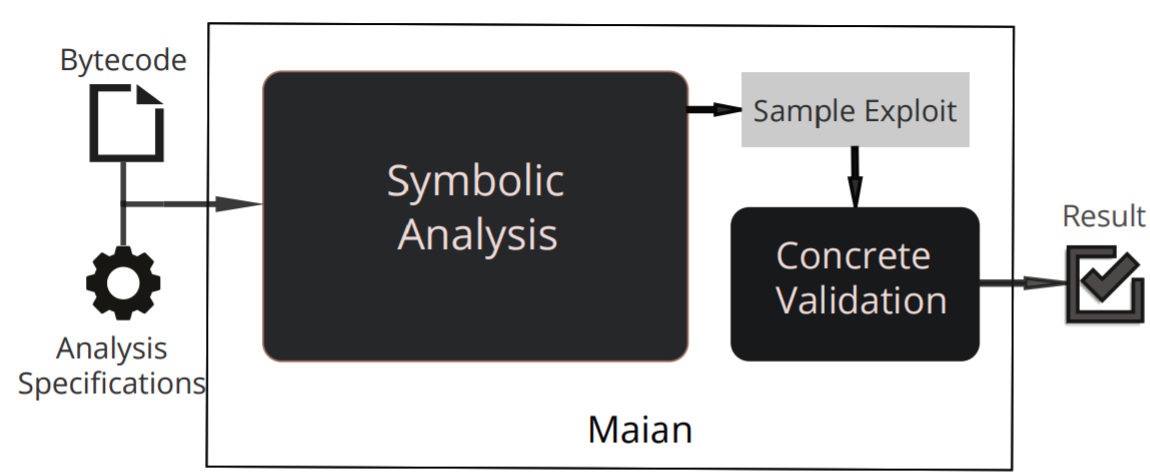
\includegraphics[scale=0.2]{MAIAN}
\end{center}
\caption{\label{fig:maian} The MAIAN Tool's Structure\cite{nikolic_kolluri_sergey_saxena_hobor_2018}}
\end{figure}

The tool introduced, MAIAN, leverages a combination of static and dynamic analysis methods as described in the introduction. It's structure is visualized in Figure~\ref{fig:maian}. It takes the Ethereum Bytecode along with analysis specifications as inputs. The analysis specification provides information about the type of vulnerabilities to search for along with other parameters to control MAIAN. MAIAN then first performs Symbolic Analysis on the given bytecode. It does this using an extension of the previously introduced OYENTE which works with traces (As OYENTE does not natively support traces). Once it detects a problematic set of inputs, it saves these and attempts to validate the exploit on a private fork of the Ethereum Network before returning it to the user to lower the number of false positives. Additionally, this execution of the potential exploit on a private fork ensures the maintenance of the state of the public Ethereum Network.

A different approach to this issue is addressed by the tool Slither developed by Feist et al. \cite{feist_grieco_groce_2019}, which uses Taint Analysis (Slither's full structure is depicted in Figure~\ref{fig:slither}). Slither functions by taking in the abstract syntax tree provided by the Solidity compiler rather than the EVM bytecode in order to preserve more information regarding the structure of the previous solidity code. Based on this extracted information, Slither converts the input to its internal representation, SlithIR, which, similar to ZEUS, is in the SSA format. In the third step, Slither performs some general analyses which can serve as a base for detecting various vulnerabilities (which can be extended by the user) in the final stage. To us, the data dependency detection is of particular interest, as Slither does this in two steps: First, Slither computes dependencies between all variables, as Securify does. Second, Slither uses Taint Analysis to mark variables which can be influenced by the user and could therefore be involved in a multi-transaction attack\footnote{It performs this Taint Analysis using function modifiers as an input as well, i.e. the dependency can be computed based on the user's privilege level, such as contract owner or regular user.}. Additionally, the authors claim it to be significantly faster and more accurate than competing analyzers.

\begin{figure}
\begin{center}
\includegraphics[scale=0.15]{Slither}
\end{center}
\caption{\label{fig:slither} The Slither Tool's Structure\cite{feist_grieco_groce_2019}}
\end{figure}


\subsubsection{Graph Construction}
Lastly, all methodologies introduced until here either ignored interactions with external smart contracts or simulated them in an inaccurate way (e.g. by marking their input as tainted or symbolically analyzing their input's possible values). In a paper by Chen et al. \cite{chen_zhu_li_chen_li_luo_lin_zhange_2018}, dynamic analysis of multiple smart contracts on the public Ethereum blockchain was conducted by creating three types of graphs, a Money Flow Graph, a Contract Creation Graph, and a Contract Invocation Graph. Using these three graphs, the authors were able to gain a better understanding of other smart contracts on the live Ethereum network.

\noindent First, given a malicious contract, the paper describes an algorithm using the Contract Creation Graph and Contract Invocation Graph to systematically detect all contracts and accounts under the control of the attacker. This methodology is useful in order to ensure that the contracts and addresses one's smart contract will interact with are not under the control of a bad actor.

\noindent Second, using the Contract Creation Graph once more, the authors provide an approach to detecting abnormal contract creation patterns, which is can be an indicator for a DoS Attack or a plot to steal tokens from a different smart contract.


\subsection{Testing}
The likely most prevalent strategy to prevent having security vulnerabilities in one's code is to write unit tests. These, however, can never detect every possible flaw, and, in the case of smart contracts, generating every dangerous state manually is exceedingly difficult. For this reason, research has gone into both Mutation Testing and fuzzing.


\subsubsection{Mutation Testing}

\noindent For the case of Mutation Testing, a paper exploring this in the context of Ethereum is by Honig et al. \cite{honig_everts_huisman_2019}. The authors introduce the Vertigo framework for Mutation Testing which runs on Truffle, a simulated Ethereum environment. This works by introducing the Solidity source code along with a working test suite to the framework. The framework then generates mutants (clones of the original contract with slight alterations in the source code) on which the test suite is run again, returning how many and which mutants passed the test suite. Based on this result, the efficacy of the test-suite can be evaluated, as described in Section~\ref{subsection:mut}.


\subsubsection{Fuzzing in Ethereum}

An automated fuzzing tool for Ethereum is called Echidna and is based on Grieco et al.'s 2020 paper \cite{grieco_song_cygan_feist_groce_2020}. Its structure is displayed in Figure~\ref{fig:echidna}. Like Vertigo, it also supports Truffle as a testing environment. Echidna takes in the smart contract source code along with a set of properties to verify and builds directly on top of the previously discussed Slither in order to gain easy access to the contracts Application binary interface (ABI) and other potentially useful constants and functions. Then, similar to Haskell's QuickCheck \cite{claessen_hughes_2000}, Echidna continuously generates random transactions conforming to the contract's ABI, previous transactions, and constants defined in the contract. If one or a combination of these violates one of the preset properties, Echidna minimizes said example and outputs it to the user.
\begin{figure}
\begin{center}
\includegraphics[scale=0.16]{echidna}
\end{center}
\caption{\label{fig:echidna} The Echidna Tool's Structure\cite{grieco_song_cygan_feist_groce_2020}}
\end{figure}

\subsection{Other}
Along with static and dynamic analysis approaches, the Ethereum ecosystem provides some other resources to aid in making smart contracts more secure: One of these is the Smart Contract Weakness Classification Registry based on EIP-1470, where one can find various examples and counterexamples to common smart contract security flaws along with testing examples ~\cite{SWC}. Another is the introduction of higher-level languages such as Obsidian ~\cite{7965268} or Vyper ~\cite{9223278}. These may not give one quite the same level of control over the EVM as Solidity does, however the greater abstraction also helps alleviate some of the flaws of Solidity. An example of these flaws is the long array of best practices concerning deprecated and dangerous operations that beginners may accidentally use, as partially described in Section~\ref{subsection:sol}.

\subsubsection{Code Metrics}
Another less formal security analysis method is the use of code metrics. Code metrics play a significant role in the Quality Assurance process of many traditional software projects which target it is to minimize bugs and maximize code quality. These two goals go hand-in-hand with maximizing security, for which reason Péter Hegedűs developed SolMet ~\cite{hegedűs_2019}. SolMet is a static analysis tool that aims to collect the same data on solidity code as tools traditionally used in QA do. Examples for this data collected by SolMet range from simple metrics such as Lines of Code to more complex metrics values like the McCabe cyclomatic complexity.

\subsection{Comparison}
Finally, we seek to compare the performance of the presented tools. The reason we seek to do this, is because although these tools often mention their performance in their respective papers, many of them have been continuously maintained and improved, meaning the metrics mentioned are outdated. Additionally, this is of interest in order to determine which tool should be prioritized over another when applying them in the industry. The tools, along with the versions of the code we used, we will compare will be Slither\cite{Slither}, OYENTE\cite{oyente}, Securify\cite{securify} and Mythril\cite{mythril}, as all of these have approximately the same goal of determining security faults. ZEUS and MAIAN, though comparable, had to be omitted, as ZEUS does not have a publicly accessible prototype and in spite of trying out multiple of MAIAN's implementation, the base was too outdated and we could not get it to run.
Echidna and Vertigo are more focused on testing, which is not directly comparable. Chen et al.'s Graph Analysis is not comparable either, as it focuses on vulnerabilities in other already deployed contract rather than finding security flaws in one's own to-be-deployed contract. Finally, formal analysis methods presented in this paper are not developed or fast enough to be comparable.

We test on a dataset \cite{data} of 114 solidity contracts, measuring the total time taken by each tool for processing these.
\begin{figure}
\centering

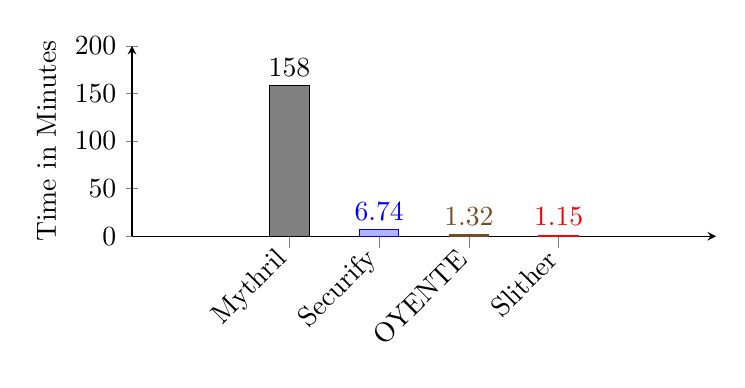
\begin{tikzpicture}
\pgfplotsset{width=10 cm}
\begin{axis} [
        symbolic x coords={ Mythril, Securify, OYENTE,Slither},
        xtick={Securify,Mythril, OYENTE, Slither},
x tick label style={rotate=45, anchor=east, align=center},
axis lines=left,
ylabel={Time in Minutes},
legend style={at={(1,-0.10)},
    anchor=north,legend columns=1},
    ybar=0pt ,
    ymin=0,
    ymax=200,
    samples=2,
    width=9cm,
    height=4cm,
    domain=1:2,
    bar width=0.5cm,
    ybar=-0.5cm,
    enlarge x limits={abs=2cm},
    nodes near coords,
    nodes near coords align={vertical},
    legend pos=north east
]
     \addplot coordinates {(Securify, 6.74)};
     \addplot coordinates {(Slither, 1.15)};
     \addplot coordinates {(OYENTE, 1.32)};
     \addplot coordinates {(Mythril, 158)};

\end{axis}
\end{tikzpicture}
\caption{Comparison of processing time for different analysis tools\label{perf:speed}}
\end{figure}



As one can see in Figure~\ref{perf:speed}, Slither and OYENTE were faster than Securify, and Mythril was significantly slower than any of its peers. However, this does not mean that Mythril is objectively worse. One reason for these performances is through the number of vulnerabilities each tool checks for: OYENTE is able to detect 4 vulnerabilities. Mythril, on the other hand, has the ability to detect more than 13 vulnerabilities. A key difference here is that Mythril is able to detect trace vulnerabilities, meaning vulnerabilities that stem from a flow of multiple transactions, as explained in Section~\ref{subsection:trace}. Detecting such vulnerabilities is significantly more time consuming. This is because in the case of Mythril, these vulnerabilities are detected by simulating multiple transactions for a single contract, which already multiplies the basic amount of work Mythril has to do compared to OYENTE. Securify detects 38 security vulnerabilities, also explaining its longer runtime compared to OYENTE. Slither, on the other hand, detects 74 security flaws, including a range of trace vulnerabilities through the means of the earlier explained Taint Analysis and still runs the fastest. Therefore, it can be conclusively said that if the only metric one considers when comparing these 4 tools is the execution speed, Slither is the best.


%-------------------------------------------------------------------------------
\section{Summary and Related Work}
%-------------------------------------------------------------------------------
All in all, we presented various methods for detecting general and Ethereum-specific security vulnerabilities.  We found that tools for static analysis and detecting attacks resulting from one transaction are very fast and very developed, along with plenty of them existing. When it comes to trace vulnerabilities multiple approaches exist in theory, however there are few easily accessible and fast tools that accurately detect these. We additionally found that the same goes for formal verification: Few tools exist employing this form of fault detection, and the ones that do are not very performant and require knowledge in proof writing to use, making them less accessible than other tools. We believe these especially yield great potential, because they have the significant benefit of being highly accurate (as they formally prove a property). Finally, there is little research like that of Chen et al. \cite{chen_zhu_li_chen_li_luo_lin_zhange_2018} concerning the security of external, already-deployed contracts that one's contract may interact with. Therefore, we believe there is still significant potential to be leveraged in the fields of trace vulnerability detection, formal analysis, and external contract checking, especially in terms of usability and accessibility for the former two. Furthermore, though out of the scope of this paper, an interesting type of security analysis would be the detection of weaknesses in smart contracts involved in Decentralized Finance, such as decentralized asset exchange contracts or decentralized loan contracts. This is of interest due to the large growth of Decentralized Finance protocols over the last year \cite{flash1}, many of which suffered significant financial loss. However, in many of these attacks, the exploit was not only a weakness in the programming logic likely stemming from a misunderstanding of how code executes in a decentralized manner (as is the case for most of the topics discussed here), but also a weakness in the understanding of how economic factors function when automated using, as explained by Cao et al. \cite{flash1} and Qin et al. \cite{flash2}, respectively. We believe, along with the improvements in current methods discussed above, the extension of existing tools to scan for these types of issues also yields great potential.

%-------------------------------------------------------------------------------
\bibliography{0-Paper}
\bibliographystyle{ieeetr}

\end{document}
